The Design Review application was implemented by using several pre-made assets.
When the application is started user is positioned into a oiltank model, which was provided by DNV GL. 
This model is of high fidelity and was originally developed for the DNV GL Survey Simulator, an application to train surveyors.

\begin{figure}%[h!] %[H]
	\frame{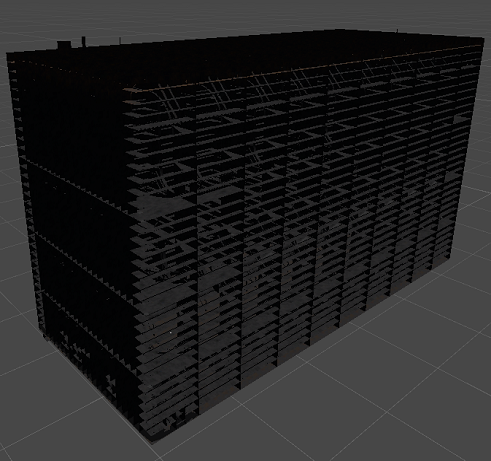
\includegraphics[width=0.5\linewidth]{pictures/screenshots/tank_back.png}}
	\frame{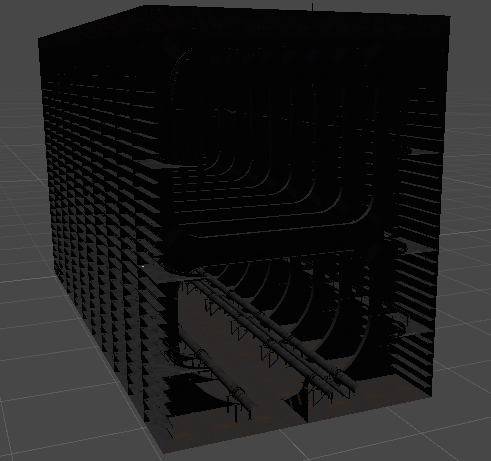
\includegraphics[width=0.5\linewidth]{pictures/screenshots/tank_half_profile.png}}
	\caption[The Oil tank model]{The Oil tank model from the outside}
	\label{fig:tank_outside}
\end{figure} 

The application also makes use of several "best practice" assets from Leap Motion, Oculus VR and SteamVR to ensure that these devices function
as optimally as possible. From Leap Motion the \texttt{LeapHandController} is utilized, which is a prefab (gameObject), with several important scripts attached to
it. Leap motion provided hand models are also being used, which was provided from the Leap Motion Hands-module. More specifically 
the \texttt{RiggedPepperCutHands} were used, but any other of the hand models could be used as easily.

From Oculus VR two prefabs is used. The first is \texttt{OVRCameraRig}, which is the recommended camera setup for using the Oculus Rift HMD. This 
prefab sets several important settings to ensure that both the head tracking and visual performance is as optimal as possible. The 
second prefab which is used is one called the \texttt{GazePointerRing}. This was showcased in a demo unity implementation by OculusVR
and is essentially a cursor that exist in the game world a fixed length in front of the user. As regular crosshair (which are drawn directly on the screen space)
isn't allowed in VR (more about this later), the \texttt{GazePointerRing} serves as a crosshair. 
From SteamVR the \texttt{[CameraRig]} prefab is used, which essentially does the same configurations as the \texttt{OVRCameraRig} does, but with the HTC Vive HMDs in mind.

The Design review application also makes use of Hover UI Kit, an open source project for creating VR/AR-enabled, customizable and dynamic user interfaces. 
This kit was vital in rapidly prototyping a gesture-enabled menu and a virtual keyboard to the annotation forms.